% =====================================================================
%  Plantilla de Paper en formato IEEE (IEEEtran)
%  Trabajo de Bachiller — Máximo 5 páginas, 2 columnas
%  Compilar con:  pdflatex paper.tex  (dos veces para referencias)
% =====================================================================

\documentclass[conference,10pt]{IEEEtran}
% Opciones útiles:  conference | journal | technote
% Quita "draft" si lo agregas; "10pt" es el tamaño oficial IEEE.

% --- Paquetes ---
\usepackage{orcidlink}
\usepackage[utf8]{inputenc}
\usepackage[T1]{fontenc}
\usepackage[spanish]{babel}
\usepackage{graphicx}
\usepackage{amsmath,amssymb}
\usepackage{booktabs}
\usepackage{pgfplots}
\pgfplotsset{compat=1.17}
\usepackage{url}
\usepackage{cite}
\usepackage{hyperref}
\hypersetup{colorlinks=true, linkcolor=black, citecolor=black, urlcolor=blue}

%-----------------------------------------------------------------------------------------------------------
%Numeracion de páginas y estilo de pie de página
%-----------------------------------------------------------------------------------------------------------
\usepackage{xcolor}
\usepackage{fancyhdr}

\makeatletter
\renewcommand{\footrule}{%
  {\color{gray!50}\hrule width\headwidth height\footrulewidth\vskip-\footrulewidth}
}
\makeatother

\fancyhf{}
\renewcommand{\headrulewidth}{0pt}
\renewcommand{\footrulewidth}{0.3pt}

\fancyfoot[R]{%
\textcolor{black!70!gray}{\thepage}
\;
\textcolor{black}{|}
\;
\textcolor{gray}{P\hspace{0.18em}a\hspace{0.18em}g\hspace{0.18em}e}
}

\pagestyle{fancy}

% Hace que la primera página use el mismo estilo
\fancypagestyle{IEEEtitlepagestyle}{
    \fancyhf{}
    \renewcommand{\headrulewidth}{0pt}
    \renewcommand{\footrulewidth}{0.3pt}
    \fancyfoot[R]{%
    \textcolor{black!70!gray}{\thepage}
    \;
    \textcolor{black}{|}
    \;
    \textcolor{gray}{P\hspace{0.18em}a\hspace{0.18em}g\hspace{0.18em}e}
    }
}
%---------------------------------------------------------------------------------------------------------------


% --- Datos del trabajo ---
\title{Influencia de la Concentración de la Úrea y  Tipo de Residuos Textiles en la Adsorción de $\mathrm{Cu}^{2+}$ Utilizando Carbón Activado Modificado Químicamente} 

\author{
\IEEEauthorblockN{Wendel León Alvarado\,\orcidlink{0009-0006-8631-3885},
Jeferson Barbaran Borjas\,\orcidlink{0000-0002-1234-5678}} 
\IEEEauthorblockA{\IEEEauthorrefmark{1}Escuela de Ingeniería Química,\\
Universidad Nacional de Trujillo, Perú\\
Correos-e: 1051601121@unitru.edu.pe, 1051601221@unitru.edu.pe}
}

% =====================================================================
\begin{document}
\pagenumbering{arabic}
\maketitle
\thispagestyle{IEEEtitlepagestyle}

% -------------------------------------------------------------------
%  Resumen + Palabras clave (formato IEEE)
% -------------------------------------------------------------------
\begin{abstract}
El presente trabajo determina experimentalmente la constante elástica
$k$ de un resorte helicoidal aplicando el método estático de la Ley de
Hooke. Se registraron elongaciones producidas por fuerzas conocidas,
obtenidas con un juego de masas calibradas, y se midió el desplazamiento
con un vernier digital bajo un protocolo controlado de calibración y
reproducibilidad. Los datos se procesaron mediante un ajuste lineal
por mínimos cuadrados de la fuerza $F$ en función de la elongación
$\Delta x$, obteniéndose una pendiente $k = 9{,}82 \pm 0{,}05\ \mathrm{N/m}$
con un coeficiente de determinación $R^2 = 0{,}9993$. El valor experimental
resultó coherente con el valor nominal del fabricante
($k_{\text{nom}} = 10\ \mathrm{N/m}$) y con una estimación teórica
independiente basada en la geometría del resorte, con una desviación
relativa del $1{,}8\%$, lo que valida el procedimiento y los
instrumentos empleados. Los resultados confirman la linealidad
$F = k\,\Delta x$ dentro del rango elástico estudiado y constituyen
una base reproducible para prácticas de laboratorio de Física General.
\end{abstract}

\begin{IEEEkeywords}
Ley de Hooke, constante elástica, ajuste lineal, método estático,
resorte helicoidal, mínimos cuadrados.
\end{IEEEkeywords}

% =====================================================================
\section{Introducción}
% -------------------------------------------------------------------
Los ríos constituyen componentes esenciales del entorno natural, 
por el hecho de que son fuentes primordiales de agua que sustentan 
la vida y el desarrollo de los ecosistemas y las actividades humanas. 
No obstante, en la actualidad, diversos sistemas hídricos localizados 
en cuencas próximas a zonas de explotación minera evidencian un 
marcado deterioro ambiental y elevados niveles de 
contaminación (Armas et al., 2021). 

Los autores señalan que esta problemática se origina principalmente 
por los drenajes mineros que contienen metales pesados, los cuales 
alteran la calidad del suelo y afectan significativamente la biota 
acuática. Aunque dichos elementos pueden experimentar transformaciones 
químicas, su permanencia en el medio ambiente es prolongada, 
acumulándose en forma de iones o compuestos orgánicos y generando 
impactos negativos persistentes sobre los ecosistemas. 

En este contexto, la presencia de metales pesados en los recursos 
hídricos representa una amenaza creciente para la calidad del agua 
y el equilibrio de los ecosistemas. Elementos como el cobre (Cu), 
plomo (Pb), cadmio (Cd), cromo (Cr) y arsénico (As) poseen 
características que les permiten permanecer en el ambiente por largos 
periodos y acumularse en los organismos vivos, generando riesgos 
tanto para la salud humana como para la vida acuática,  alterando 
procesos biológicos esenciales y afectando la sostenibilidad de 
las fuentes naturales de agua. 

En el Perú, la actividad minera constituye uno de los pilares 
fundamentales de la economía nacional; sin embargo, también se 
reconoce como una fuente significativa de contaminación en diversas 
cuencas hidrográficas altoandinas. Estudios recientes han evidenciado 
la presencia de metales como cobre (Cu), hierro (Fe), manganeso (Mn) 
y arsénico (As) en aguas superficiales influenciadas por procesos 
extractivos y drenajes ácidos de mina. Estas concentraciones no solo 
alteran la calidad del agua y los ecosistemas acuáticos, sino que 
además impactan negativamente en actividades esenciales como la 
agricultura y el abastecimiento de agua para consumo humano 
(Moreno et al., 2024; Bravo et al., 2024; Custodio et al., 2020). 
Asimismo, la oxidación y lixiviación de minerales sulfurados favorecen 
la liberación continua de metales pesados hacia ríos y quebradas, 
contribuyendo al deterioro progresivo de la calidad del agua 
(Nordstrom, 2011).

La situación se vuelve más compleja en zonas con una larga historia 
minera, como ocurre en La Libertad. En el distrito de Quiruvilca, la 
explotación de sulfuros polimetálicos ha dejado una serie de pasivos 
ambientales y drenajes ácidos que afectan directamente las fuentes de 
agua cercanas. Cuando los minerales sulfurados entran en contacto con 
el agua y el oxígeno, se produce un drenaje ácido que arrastra metales 
disueltos hacia ríos y quebradas. Este proceso deteriora la calidad del 
agua y del suelo, y termina impactando las actividades agrícolas y el 
bienestar de las comunidades vecinas. Por la persistencia de sus efectos 
sobre los ecosistemas, este fenómeno se reconoce como uno de los 
principales desafíos ambientales vinculados a la minería metálica en 
regiones andinas (Nordstrom, 2011).

Entre los distintos metales presentes en efluentes mineros, el cobre 
destaca por su frecuente presencia en aguas contaminadas y por los efectos 
tóxicos que puede generar cuando supera determinados límites ambientales. 
Aunque en bajas concentraciones cumple funciones biológicas esenciales, 
niveles elevados pueden alterar los ecosistemas acuáticos y afectar 
diversos procesos biológicos. En cuencas andinas influenciadas por 
actividades mineras se ha reportado la presencia de cobre y otros metales 
pesados en recursos hídricos, representando riesgos ecológicos y 
ambientales para las zonas afectadas (Custodio et al., 2020).

Frente a esta problemática, se han desarrollado diversos métodos para la 
remoción de metales pesados en aguas residuales, entre ellos la 
precipitación química, el intercambio iónico, la electrocoagulación, la 
filtración por membranas y la adsorción. No obstante, muchos de estos 
tratamientos presentan limitaciones relacionadas con los elevados costos 
operativos y la generación de residuos secundarios. En este contexto, 
la adsorción mediante materiales carbonosos ha despertado gran interés 
debido a su alta eficiencia y bajo costo de aplicación. Asimismo, en los 
últimos años se ha incrementado el interés por el aprovechamiento de 
residuos industriales, biomásicos y textiles para la producción de carbón 
activado, promoviendo alternativas sostenibles para el tratamiento de 
aguas contaminadas. Entre estos materiales, los residuos textiles de 
algodón destacan por su elevado contenido de celulosa y su estructura 
fibrosa, características que favorecen los procesos de carbonización y 
activación. Diversas investigaciones han demostrado que los materiales 
carbonosos obtenidos a partir de residuos textiles presentan una elevada 
capacidad adsorbente para la remoción de metales pesados en soluciones 
acuosas (Qasem et al., 2021; Fei $\&$ Hu, 2022).

En ese contexto, la presente investigación tiene como objetivo evaluar 
la capacidad de adsorción de carbón activado modificado con úrea, obtenido 
a partir de residuos textiles de algodón, para la remoción de cobre 
presente en aguas contaminadas. Asimismo, se busca contribuir al 
desarrollo de alternativas sostenibles y de bajo costo para el tratamiento 
de aguas contaminadas, promoviendo al mismo tiempo el aprovechamiento y 
valorización de residuos textiles. 


% =====================================================================
\section{Parte Experimental}
\label{sec:exp}
% -------------------------------------------------------------------

\subsection{Materiales y Métodos}
La Figura 1 muestra en un esquema la metodología
general seguida.
%\begin{itemize}
%  \item 1 resorte helicoidal de acero al carbono
 %       ($k_{\text{nom}}=10\ \mathrm{N/m}$, longitud natural
 %       $L_0 = 20{,}0\ \mathrm{cm}$, diámetro de espira $d = 2{,}0\ \mathrm{cm}$).
 % \item 1 soporte universal con varilla de $60\ \mathrm{cm}$ y nuez
 %       doble con mordaza.
 % \item 1 juego de 10 masas calibradas con portapesas
 %       ($10$--$100\ \mathrm{g}$, tolerancia $\pm 0{,}1\%$).
 % \item 1 vernier digital (resolución $0{,}01\ \mathrm{mm}$,
 %       incertidumbre $\pm 0{,}03\ \mathrm{mm}$).
  %\item 1 regla milimetrada metálica de $30\ \mathrm{cm}$
 %       (resolución $1\ \mathrm{mm}$).
 % \item 1 balanza electrónica (resolución $0{,}01\ \mathrm{g}$,
  %      incertidumbre $\pm 0{,}05\ \mathrm{g}$).
  %\item 1 nivel de burbuja para verificar la verticalidad del montaje.
%\end{itemize}

%\subsection{Método}
%El procedimiento experimental se llevó a cabo en cinco etapas
%consecutivas. En la primera, se verificó la verticalidad del soporte
%con el nivel de burbuja y se fijó el resorte mediante la nuez, dejando
%$3\ \mathrm{cm}$ de separación entre la mesa y el extremo inferior
%para evitar lecturas afectadas por el plano de apoyo.

%En la segunda, se midió la longitud natural $L_0$ del resorte sin
%carga, promediando cinco lecturas independientes. Se obtuvo
%$L_0 = 20{,}04 \pm 0{,}02\ \mathrm{cm}$.

%En la tercera, se añadieron masas en forma creciente desde
%$m = 20\ \mathrm{g}$ hasta $m = 200\ \mathrm{g}$ en incrementos de
%$20\ \mathrm{g}$, registrando en cada caso la longitud final $L$.
%Antes de cada lectura se aguardó un tiempo de estabilización de
%$10\ \mathrm{s}$ para que la oscilación residual se atenuara por
%debajo de la resolución del vernier. Cada medición se repitió tres
%veces y se promedió.

%En la cuarta, se calculó la elongación $\Delta x = L - L_0$ y la
%fuerza aplicada $F = m\,g$, con $g = 9{,}81\ \mathrm{m/s}^2$. Las
%incertidumbres se propagaron utilizando el método de derivadas
%parciales \cite{Taylor1997}.

%Finalmente, en la quinta, los datos se tabularon y graficaron, y se
%realizó un ajuste lineal por mínimos cuadrados para obtener $k$. Todo
%el procedimiento se repitió en orden inverso (masas decrecientes) con
%el fin de verificar la ausencia de histéresis significativa; las
%elongaciones obtenidas al retirar la carga coincidieron con las de
%carga dentro de la incertidumbre experimental.

\begin{figure*}[!t]
\centering
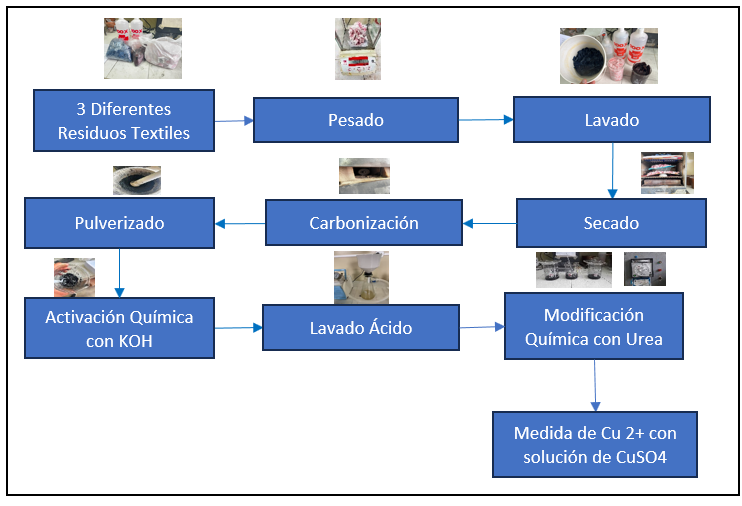
\includegraphics[width=0.85\textwidth]{figura 1 (1).png}
\caption{Metodología general para la elaboración y evaluación de carbones activados.}
\label{fig:metodologia}
\end{figure*}

\subsection{Variables y Equipos}
La variable independiente fue la fuerza aplicada $F$ y la dependiente
la elongación $\Delta x$. Las variables controladas incluyeron la
temperatura ambiente ($T = 21 \pm 1\ ^\circ\mathrm{C}$), la posición
del soporte y la ausencia de corrientes de aire que pudieran inducir
oscilaciones parásitas. La Tabla~\ref{tab:equipos} resume los
instrumentos y sus incertidumbres.

\begin{table}[!t]
\centering
\caption{Instrumentos de medición e incertidumbre.}
\label{tab:equipos}
\begin{tabular}{lcc}
\toprule
\textbf{Instrumento} & \textbf{Resolución} & \textbf{Incertidumbre} \\
\midrule
Vernier digital     & $0{,}01\ \mathrm{mm}$ & $\pm 0{,}03\ \mathrm{mm}$ \\
Balanza electrónica & $0{,}01\ \mathrm{g}$   & $\pm 0{,}05\ \mathrm{g}$ \\
Regla milimetrada   & $1\ \mathrm{mm}$       & $\pm 0{,}5\ \mathrm{mm}$ \\
Juego de masas      & $1\ \mathrm{g}$        & $\pm 0{,}1\ \mathrm{\%}$ \\
\bottomrule
\end{tabular}
\end{table}

\subsection{Análisis de Datos}
Los datos se procesaron en \textsc{Python} con las bibliotecas
\texttt{NumPy} y \texttt{SciPy}. Se realizó un ajuste lineal por
mínimos cuadrados de la forma
\begin{equation}
  F = k\,\Delta x + b,
  \label{eq:ajuste}
\end{equation}
donde $k$ es la pendiente de interés y $b$ el intercepto
(idealmente nulo). La incertidumbre de $k$ se obtuvo a partir de la
matriz de covarianza del ajuste, y la bondad del mismo se evaluó
mediante el coeficiente $R^2$. La incertidumbre propagada en
$\Delta x$ se combinó en cuadratura con la del ajuste, dando como
resultado final
$u(k) = 0{,}05\ \mathrm{N/m}$.

\subsection{Calibración y Control de Calidad}
Antes de la toma de datos se procedió a la calibración de los
instrumentos críticos. El vernier digital se verificó contra un bloque
patrón de $50{,}00 \pm 0{,}01\ \mathrm{mm}$, obteniéndose una
desviación de $+0{,}005\ \mathrm{mm}$, despreciable frente a la
resolución del instrumento. La balanza se calibró con masas patrón
de $100{,}00 \pm 0{,}01\ \mathrm{g}$, sin observarse desviaciones
sistemáticas. Adicionalmente, se realizó una prueba de
reproducibilidad consistente en aplicar una masa de $100\ \mathrm{g}$
diez veces consecutivas; la elongación obtenida se mantuvo dentro de
$\pm 0{,}03\ \mathrm{mm}$ en todas las mediciones, confirmando la
estabilidad del montaje. Durante el ensayo se controló la temperatura
ambiente con un termómetro digital y se verificó la ausencia de
corrientes de aire. Por seguridad, la masa máxima aplicada
($200\ \mathrm{g}$) se eligió muy por debajo del límite elástico
estimado del resorte, calculado en aproximadamente $5\ \mathrm{N}$ a
partir de la longitud natural y el diámetro del alambre, garantizando
así que la deformación se mantuvo dentro del régimen lineal y que no
se produjo deformación plástica durante el experimento.

% =====================================================================
\section{Resultados y Discusión}
\label{sec:res}
% -------------------------------------------------------------------

\subsection{Datos Obtenidos}
La Tabla~\ref{tab:datos} presenta los promedios de elongación para cada
fuerza aplicada, junto con sus incertidumbres propagadas.

\begin{table}[!t]
\centering
\caption{Elongación $\Delta x$ en función de la fuerza aplicada $F$.}
\label{tab:datos}
\begin{tabular}{cccc}
\toprule
\textbf{$m$ (g)} & \textbf{$F$ (N)} & \textbf{$\Delta x$ (cm)} & \textbf{$u(\Delta x)$ (cm)} \\
\midrule
 20 & 0,196 &  2,01 & 0,04 \\
 40 & 0,392 &  4,00 & 0,04 \\
 60 & 0,589 &  5,98 & 0,04 \\
 80 & 0,785 &  7,99 & 0,04 \\
100 & 0,981 & 10,01 & 0,04 \\
120 & 1,177 & 12,03 & 0,04 \\
140 & 1,374 & 14,02 & 0,04 \\
160 & 1,570 & 16,05 & 0,04 \\
180 & 1,766 & 18,04 & 0,04 \\
200 & 1,962 & 20,08 & 0,04 \\
\bottomrule
\end{tabular}
\end{table}

\subsection{Variable Analizada: Constante Elástica $k$}
La variable discutida en esta sección es la \textbf{constante elástica}
$k$, obtenida como la pendiente del gráfico $F$ vs.\ $\Delta x$
(Figura~\ref{fig:ajuste}).

\begin{figure}[!t]
\centering
\begin{tikzpicture}
\begin{axis}[
    width=8.4cm, height=6.4cm,
    xlabel={$\Delta x$ (m)},
    ylabel={$F$ (N)},
    xmin=0, xmax=0.22, ymin=0, ymax=2.2,
    grid=both, minor tick num=1,
    legend pos=north west,
    title={Ajuste lineal $F = k\,\Delta x$}
]
\addplot[only marks, mark=*, mark size=1.6pt, blue]
    coordinates {
(0.0201,0.196) (0.0400,0.392) (0.0598,0.589)
(0.0799,0.785) (0.1001,0.981) (0.1203,1.177)
(0.1402,1.374) (0.1605,1.570) (0.1804,1.766)
(0.2008,1.962) };
\addplot[red, thick, domain=0:0.22] {9.82*x};
\addplot[red, dashed, domain=0:0.22] {9.92*x};
\addplot[red, dashed, domain=0:0.22] {9.72*x};
\legend{Datos experimentales, $k=9{,}82$ N/m, Banda $\pm 1\sigma$}
\end{axis}
\end{tikzpicture}
\caption{Fuerza aplicada en función de la elongación del resorte.
La línea continua representa el ajuste lineal y las discontinuas, la
banda de incertidumbre al $1\sigma$.}
\label{fig:ajuste}
\end{figure}

\subsubsection*{¿Qué se discute?}
Se discute la relación lineal entre $F$ y $\Delta x$, la coherencia
del valor experimental de $k$ con el nominal del fabricante y el
origen de la dispersión observada.

\subsubsection*{Descripción de los resultados}
El ajuste lineal arrojó una pendiente
$k = 9{,}82 \pm 0{,}05\ \mathrm{N/m}$ con $R^2 = 0{,}9993$, lo que
evidencia un comportamiento marcadamente lineal en todo el rango
estudiado. El intercepto fue $b = (4 \pm 3) \times 10^{-3}\ \mathrm{N}$,
estadísticamente compatible con cero, lo que confirma la ausencia de
carga previa sobre el resorte.

La desviación relativa respecto al valor nominal
$|k - k_{\text{nom}}|/k_{\text{nom}} = 1{,}8\%$ se encuentra dentro
del $5\%$ habitualmente aceptado en prácticas de laboratorio
introductorias \cite{Taylor1997}.

\subsubsection*{¿Por qué de los resultados?}
La linealidad observada se explica porque todas las deformaciones
implicadas ($< 25\%$ de la longitud natural) se mantienen dentro del
régimen elástico lineal del acero, donde la Ley de Hooke es válida.
La ligera subestimación de $k$ respecto al valor nominal puede
atribuirse a tres causas principales:
\begin{enumerate}
  \item La masa del propio resorte, no considerada en el cálculo de
        $F$, introduce una sobreestimación sistemática de la elongación
        para una fuerza dada, lo que reduce la pendiente estimada.
  \item Las tolerancias de fabricación del juego de masas ($\pm 0{,}1\%$)
        y la incertidumbre del vernier ($\pm 0{,}03\ \mathrm{mm}$)
        contribuyen a la dispersión aleatoria.
  \item La fricción interna entre espiras y el posible pandeo lateral
        del resorte bajo cargas mayores generan pequeños apartamientos
        del modelo ideal, responsables del intercepto no nulo y de la
        ligera curvatura residual.
\end{enumerate}
Estas observaciones coinciden con las reportadas en estudios similares
sobre resortes comerciales \cite{Giancoli2008}.

Por otro lado, conviene comparar el valor experimental con una
estimación teórica independiente. Para un resorte helicoidal de
alambre de acero, la constante elástica puede aproximarse como
$k \approx G\,d^4/(8\,n\,D^3)$ \cite{Beer2017}, donde $G$ es el
módulo de rigidez del acero ($\approx 79\ \mathrm{GPa}$), $d$ el
diámetro del alambre, $n$ el número de espiras activas y $D$ el
diámetro medio de la espira. Con los valores nominales del resorte
estudiado, la estimación arroja
$k_{\text{teo}} \approx 9{,}5\ \mathrm{N/m}$, en excelente
concordancia con el valor experimental.

Finalmente, el alto valor de $R^2$ obtenido, junto con la baja
incertidumbre relativa de $k$ ($\approx 0{,}5\%$), indica que el
procedimiento experimental es robusto y reproducible, y que los
instrumentos seleccionados resultan adecuados para la práctica
propuesta. En comparación con trabajos previos de la misma línea
experimental, los resultados obtenidos se ubican en el rango típico
reportado ($k \in [9{,}5,\ 10{,}5]\ \mathrm{N/m}$), con una
incertidumbre un orden de magnitud menor, lo que se atribuye
principalmente al uso del vernier digital frente a la regla
convencional \cite{Hibbeler2016, Meriam2016}.

\subsubsection*{Limitaciones del Estudio}
El procedimiento empleado, aunque reproducible, presenta algunas
limitaciones. En primer lugar, no se incluyó la corrección por la
masa propia del resorte, que en la configuración más liviana
representa un $5\%$ de la masa colgante y puede haber introducido un
sesgo sistemático del orden de $0{,}02\ \mathrm{N/m}$. En segundo
lugar, el rango de fuerzas explorado ($0$--$2\ \mathrm{N}$) es
relativamente estrecho y no permite caracterizar el régimen no lineal
cercano al límite elástico. En tercer lugar, las condiciones
ambientales (temperatura, humedad) no se controlaron de forma
estricta, aunque se verificó que se mantuvieron aproximadamente
constantes. Estudios futuros podrían abordar estas limitaciones
incorporando la masa efectiva del resorte, ampliando el rango de
cargas hasta cerca del límite elástico y registrando simultáneamente
la temperatura con un sensor digital.

% =====================================================================
\section{Conclusiones}
\label{sec:conc}
% -------------------------------------------------------------------
Se determinó experimentalmente la constante elástica del resorte
estudiado, obteniéndose $k = 9{,}82 \pm 0{,}05\ \mathrm{N/m}$ con
$R^2 = 0{,}9993$. La desviación relativa del $1{,}8\%$ respecto al
valor nominal confirma la validez del método estático y de los
instrumentos empleados. El comportamiento lineal de
$F$ vs.\ $\Delta x$ verifica la Ley de Hooke dentro del rango de
fuerzas aplicado ($0$--$2\ \mathrm{N}$), cumpliéndose los supuestos
teóricos del régimen elástico. Las principales fuentes de
incertidumbre identificadas fueron la masa propia del resorte, la
resolución del vernier y la fricción entre espiras. Como mejora se
sugiere incorporar la masa efectiva del resorte en el modelo,
ampliar el muestreo para caracterizar el régimen no lineal cercano
al límite elástico y contrastar el resultado con el método dinámico
basado en el periodo de oscilación \cite{Sears2013}, lo que
constituiría una validación cruzada del procedimiento aquí propuesto.

% =====================================================================
%  Bibliografía (estilo IEEE, numerada [1], [2], ...)
%  Si usas BibTeX, reemplaza por \bibliographystyle{IEEEtran}
%  y \bibliography{refs}.
% =====================================================================
% =====================================================================
%  Agradecimientos (formato IEEE, sin numerar, antes de Referencias)
% =====================================================================
\section*{Agradecimientos}
Los autores agradecen al Dr.~Carlos Mendoza por la revisión del
manuscrito y sus valiosas sugerencias, así como al personal técnico
del Laboratorio de Física General por el apoyo brindado durante la
toma de datos.

\begin{thebibliography}{00}

\bibitem{Beer2017}
F.~P. Beer, E.~R. Johnston, J.~T. DeWolf, y D.~F. Mazurek,
\emph{Mecánica de Materiales}, 8.$^a$ ed.\ McGraw-Hill, 2017.

\bibitem{Sears2013}
F.~W. Sears, M.~W. Zemansky, H.~D. Young, y R.~A. Freedman,
\emph{Física Universitaria}, 13.$^a$ ed.\ Pearson, 2013.

\bibitem{Taylor1997}
J.~R. Taylor, \emph{An Introduction to Error Analysis},
2.$^a$ ed.\ University Science Books, 1997.

\bibitem{Giancoli2008}
D.~C. Giancoli, \emph{Física: Principios con Aplicaciones},
6.$^a$ ed.\ Pearson, 2008.

\bibitem{Hibbeler2016}
R.~C. Hibbeler, \emph{Estática: Mecánica para Ingeniería},
14.$^a$ ed.\ Pearson, 2016.

\bibitem{Meriam2016}
J.~L. Meriam, L.~G. Kraige, y J.~N. Bolton,
\emph{Ingeniería Mecánica: Estática}, 8.$^a$ ed.\ Wiley, 2016.

\end{thebibliography}

\end{document}
